\documentclass[11pt]{article}
\usepackage{amsmath}
\usepackage[margin=0.68in]{geometry}
\usepackage{booktabs}
\usepackage[american]{circuitikz}
\usepackage{enumitem}
\usepackage{fancyhdr}
\usepackage{graphicx}
\usepackage[table]{xcolor}
\usepackage[hidelinks]{hyperref}
\usepackage{listings}
\usepackage{microtype}
\usepackage{tabularx}
\usepackage{titlesec}
\graphicspath{{docs/lessons/assets/}{../assets/}}
\definecolor{Ink}{gray}{0}
\definecolor{CodeGray}{gray}{0.96}
\hypersetup{hidelinks,pdftitle={ADK Lesson 038: Acoustic Envelope},
 pdfauthor={Kevin Shanahan},
 pdfsubject={Deterministic baseline, acoustic event windows, clipping, and relative evidence},
 pdflang={en-US}}
\pagestyle{fancy}\fancyhf{}
\lhead{\textsc{ADK Lesson 038}}\rhead{Acoustic Envelope}
\cfoot{\thepage}\setlength{\headheight}{14pt}
\setlength{\parindent}{0pt}\setlength{\parskip}{5pt}
\setlist{nosep,leftmargin=1.45em}
\titleformat{\section}{\Large\bfseries\color{Ink}}{\thesection}{0.5em}{}
\lstdefinestyle{adkcpp}{language=C++,backgroundcolor=\color{CodeGray},
 basicstyle=\ttfamily\small,keywordstyle=\color{Ink}\bfseries,
 commentstyle=\color{Ink},columns=fullflexible,keepspaces=true,
 showstringspaces=false,frame=single,rulecolor=\color{Ink},
 breaklines=true,tabsize=4}
\newcommand{\lessonbox}[1]{%
 \begin{center}\fcolorbox{Ink}{white}{\parbox{0.92\linewidth}{#1}}\end{center}}

\begin{document}
\begin{center}
 {\Huge\bfseries Acoustic Envelope}\\[4pt]
 {\Large Turn supplied samples into one bounded event window}\\[8pt]
 \textit{Calibrate quiet, retain a peak, publish relative evidence}
\end{center}
\begin{tabularx}{\linewidth}{@{}>{\bfseries}l X >{\bfseries}l X@{}}
Lesson & 038 --- component & Time & 120--180 minutes\\
Prerequisites & Lessons 007, 012, and 037 & Board & Mega 2560\\
Evidence & trace fixture and three LEDs & Status & host verified; bench open\\
Energy class & E0 copied observations; provisional E1 reference fixture\\
\end{tabularx}

\lessonbox{\textbf{Scope gate.} This lesson interprets supplied
\texttt{ENVELOPE} and optional \texttt{GATE} samples. It records no waveform,
audio, or speech and makes no claim about sound-pressure level (SPL), loudness,
frequency, source identity, hearing, impact severity, alarms, or surveillance.
The optional physical route is only the SparkFun SEN-12642 with visible
\texttt{V10} silkscreen matched to the pinned hardware V1.0 sources.}

\section{Mission and vocabulary}
The evidence chain is:
\[
\text{supplied ADC/threshold trace}\rightarrow\text{quiet baseline}
\rightarrow\text{event window}\rightarrow\text{unitless intensity}.
\]
\texttt{AcousticEnvelope} is a pure behavior. It owns no endpoint, pin,
interrupt, sampling timer, ADC reference, heap, callback, or hidden clock.
The caller copies one ADC sample and, when configured, one threshold sample
into each timestamped frame. The canonical sketch defaults to a deterministic
trace, so the complete software experiment requires no acoustic hardware.

\section{Read the exact reference circuit}
The optional reference detector, Mega, and USB source share one 5 V powered
and unpowered state. Connect \texttt{ENVELOPE} to A0 at \textbf{TP-E};
connect active-high \texttt{GATE} to D22 at \textbf{TP-T} with no input
pull-up. Leave \texttt{AUDIO} disconnected. The Mega ADC uses AVcc as its
reference. D30, D31, and D32 each drive one LED through 1 k\(\Omega\) to GND.

\begin{center}
% ADK visual: schematic
\begin{circuitikz}[american voltages]
  \draw (0,4.5) node[left]{Mega 5 V} to[short,o-] (1.2,4.5)
    -- (3.0,4.5) node[right]{SEN-12642 V10 VCC};
  \draw (0,3.7) node[left]{Mega GND} to[short,o-] (1.2,3.7)
    -- (3.0,3.7) node[right]{SEN-12642 V10 GND};
  \draw (3.0,2.8) node[left]{ENVELOPE} -- (5.0,2.8)
    node[above]{TP-E} -- (7.0,2.8) node[right]{Mega A0};
  \draw (3.0,2.0) node[left]{GATE} -- (5.0,2.0)
    node[above]{TP-T} -- (7.0,2.0) node[right]{Mega D22, no pull};
  \draw (3.0,1.4) node[left]{AUDIO} to[short,-o] (4.2,1.4)
    node[right]{NC};
  \draw (0,0) node[left]{Mega D30}
    to[R,l={1 k\(\Omega\)},o-] (3.2,0)
    to[leD] (4.8,0) -- (5.2,0) node[right]{event evidence};
  \draw (5.0,0) -- (5.0,-0.3) node[ground]{};
  \draw (0,-0.8) node[left]{Mega D31}
    to[R,l={1 k\(\Omega\)},o-] (3.2,-0.8)
    to[leD] (4.8,-0.8) -- (5.2,-0.8) node[right]{gate evidence};
  \draw (5.0,-0.8) -- (5.0,-1.1) node[ground]{};
  \draw (0,-1.6) node[left]{Mega D32}
    to[R,l={1 k\(\Omega\)},o-] (3.2,-1.6)
    to[leD] (4.8,-1.6) -- (5.2,-1.6) node[right]{ready/fault evidence};
  \draw (5.0,-1.6) -- (5.0,-1.9) node[ground]{};
\end{circuitikz}

\small\textit{Electrically authoritative connection schematic for the named
V10 reference fixture. D30, D31, and D32 are three independent branches; no
LED, resistor, or node is shared.}
\end{center}

This circuit does not authorize a look-alike sound board, KY-037/KY-038, or an
unknown Elegoo module. Before power, match the visible V10 revision, trace the
common ground, confirm \texttt{AUDIO} is open, and inspect for damage. The
detector must never remain powered while the Mega is unpowered.

\section{Read the supplied trace}
\begin{center}
% ADK visual: pencil
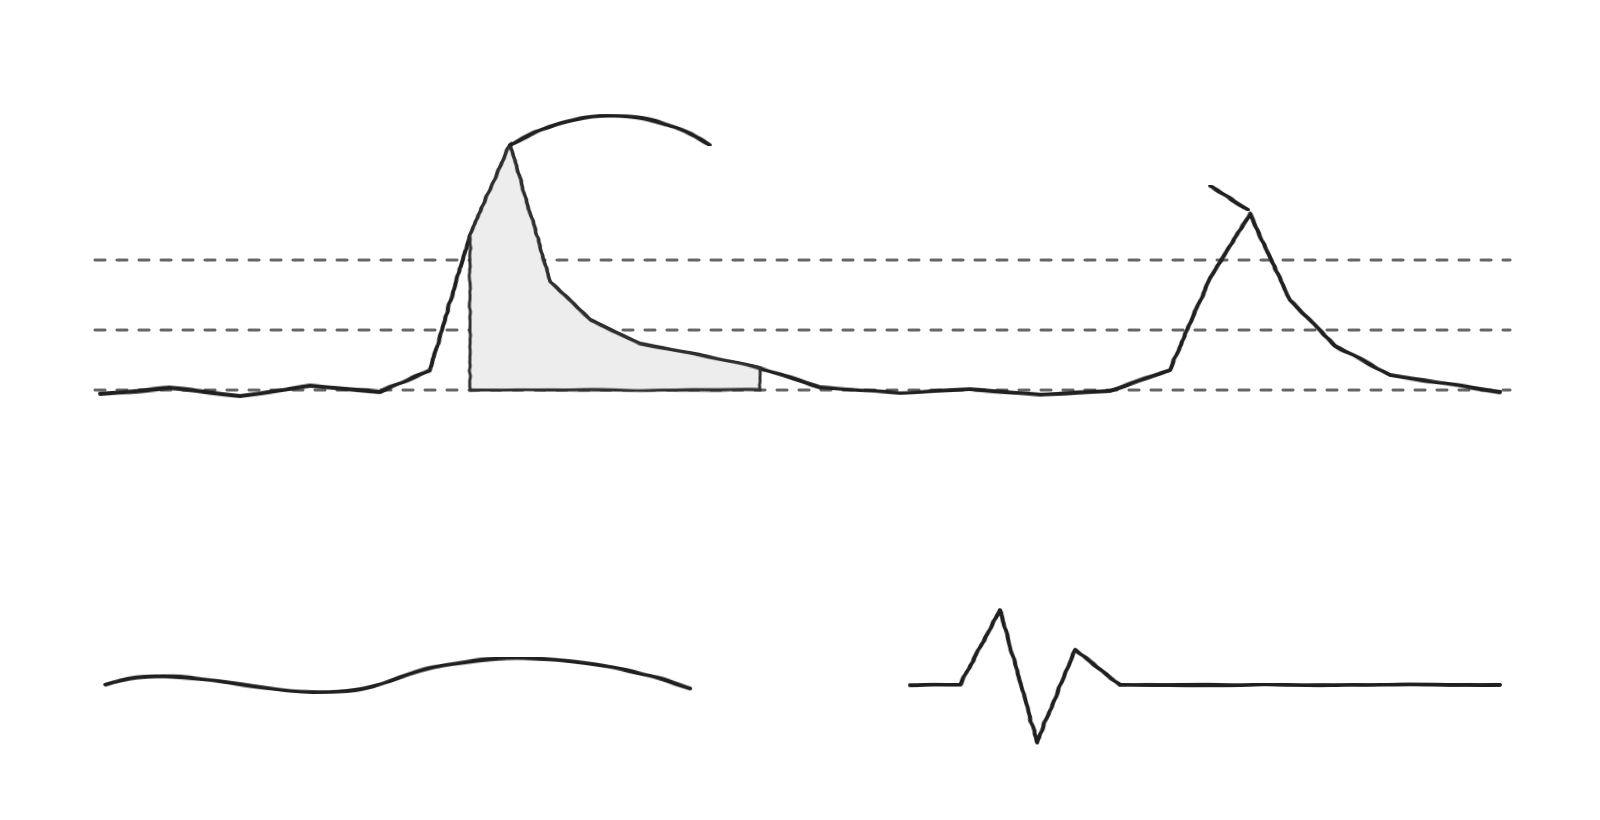
\includegraphics[width=0.98\linewidth]{038-envelope-trace-pencil.png}

\small\textit{Alternative text: a pencil ADC trace settles around a quiet
baseline, crosses a configured attack offset, retains one peak, and closes
after continuous quiet at a smaller release offset; a separate sparse trace
shows that activity between supplied sample times may be missed.}

\small Dashed lines, from low to high, mark baseline, release, and attack.
Vertical strokes mark event start and quiet close; the shaded region is the
bounded event window. The lower strokes contrast slow quiet adaptation with a
narrow excursion between supplied samples.
\end{center}

The first healthy, non-clipped sample establishes the baseline and starts
calibration with zero amplitude. During calibration and quiet, the integer
estimate follows:
\[
B_{\mathrm{next}}=B+\operatorname{trunc}\!\left(
\frac{\text{raw}-B}{2^{\texttt{baselineShift}}}\right).
\]
It freezes while an event or refractory interval is active. Each amplitude is
\(\lvert\text{raw}-B\rvert\). Attack requires amplitude at least the configured
attack offset; release requires amplitude at most the smaller release offset.
That gap prevents one noisy boundary from repeatedly opening and closing.

Calibration includes the first sample at or beyond its configured duration.
Before that boundary, no event is qualified. A rail sample before calibration
starts does not establish a baseline; clipping during calibration faults and
requires reset.

\section{Open, retain, and close one event}
An attack opens one bounded window and freezes the baseline. The window retains
the greatest observed amplitude. It closes at the earlier of continuous quiet
for \texttt{quietToClose} or exact \texttt{eventWindow} expiry. Refractory time
starts at completion and blocks another event until its exact boundary.

Only the completion update publishes relative intensity. Define:
\[
H=\max(B-\texttt{railMargin},(1023-\texttt{railMargin})-B).
\]
For peak \(P\), attack offset \(A\), and valid \(H>A\):
\[
I=
\frac{1000\cdot\operatorname{clamp}(P-A,0,H-A)}{H-A}.
\]
Integer division truncates. \(I\) is exact replay evidence in the range
0--1000 for this configuration and baseline. It is unitless: do not compare it
to dB SPL, another board, another gain setting, another baseline, or another
room as though those values share a physical scale.

\begin{tabularx}{\linewidth}{@{}l X@{}}
\toprule
Published field & Interpretation\\
\midrule
\texttt{raw}, \texttt{baseline}, \texttt{amplitude} & current supplied sample and derived offset\\
\texttt{peakAmplitude} & largest supplied amplitude in the open window\\
\texttt{eventStarted/Completed} & one-update transition evidence\\
\texttt{eventStartedAt/Duration} & bounded interval over supplied timestamps\\
\texttt{relativeIntensity} & completed-event value, 0--1000, unitless\\
\texttt{phase/quality/status} & whether any of the above is qualified\\
\bottomrule
\end{tabularx}

\section{Confidence before interpretation}
\begin{center}
% ADK visual: pencil
\begin{tikzpicture}[x=0.0006125\linewidth,y=0.0006125\linewidth]
\node[anchor=south west,inner sep=0] at (0,0)
% ADK visual: pencil
 {
\includegraphics[width=0.98\linewidth]{038-confidence-pencil.png}};
\node[font=\sffamily\scriptsize] at (215,558) {supplied sample};
\node[font=\sffamily\scriptsize] at (615,558) {quiet calibration};
\node[font=\sffamily\scriptsize] at (1020,558) {open event};
\node[font=\sffamily\scriptsize] at (1407,558) {0--1000 result};
\node[font=\sffamily\scriptsize] at (215,298) {source fault};
\node[font=\sffamily\scriptsize] at (615,298) {rail clipping};
\node[font=\sffamily\tiny] at (1020,298) {threshold disagreement};
\node[font=\sffamily\scriptsize] at (1395,298) {refractory hold};
\node[font=\sffamily\scriptsize] at (430,85)
 {bounded relative evidence --- not SPL};
\end{tikzpicture}

\small\textit{Alternative text: a pencil flow runs from a supplied ADC and
optional threshold sample through quiet calibration and an event window to a
unitless 0--1000 result; side branches stop for source failure, rail clipping,
sustained threshold disagreement, and refractory time.}

\small Top row, left to right: supplied sample, quiet calibration, open event,
unitless result. Downward branches, left to right: source fault, rail clipping,
sustained threshold disagreement, and refractory hold.
\end{center}

\texttt{raw <= railMargin} is \texttt{ClippedLow};
\(\texttt{raw >= 1023-railMargin}\) is \texttt{ClippedHigh}. Clipping cannot
open or extend an event. A failed analog source is not interpreted at all. A
configured threshold source must also be healthy.

After calibration, the optional digital threshold is compared with the
analog authority: active should agree with amplitude at or above attack.
One mismatch is visible evidence, not a fault. Continuous mismatch for
\texttt{quietToClose} becomes \texttt{ThresholdDisagreement}. Comparator
output never replaces the analog envelope for timing or intensity, and a
threshold-only specimen is unsupported.

\begin{tabularx}{\linewidth}{@{}l l l X@{}}
\toprule
Phase & Quality & Status & Event-field rule\\
\midrule
Calibrating & Unqualified & Ok & event fields canonical zero\\
Quiet & ValidQuiet & Ok & event fields canonical zero\\
EventOpen & ValidEvent & Ok & live start/peak; completion and intensity false/zero\\
Refractory & ValidEvent & Ok & completion update publishes nonzero duration\\
Refractory & ValidQuiet & Ok & completion snapshot cleared; no new attack\\
Fault & ClippedLow/High & InvalidArgument & event and intensity fields cleared\\
Fault & ThresholdDisagreement & HardwareFailure & event and intensity fields cleared\\
Fault & SourceFault & exact source status & event and intensity fields cleared\\
Fault & SourceFault & HardwareFailure & configured threshold presence mismatch; event/intensity cleared\\
Fault & SourceFault & InvalidArgument & malformed runtime threshold enum; event/intensity cleared\\
Fault & TimingFault & InvalidArgument & last completed evidence retained\\
Fault & Unqualified & InvalidArgument & raw above 1023 or invalid headroom; event/intensity cleared\\
\bottomrule
\end{tabularx}

No other phase, quality, and status tuple is legal. ``Exact source status''
means the non-Ok analog status, or the configured threshold status after a
healthy analog sample. A malformed runtime threshold \texttt{Level} is instead
\texttt{Fault/SourceFault/InvalidArgument}. A supplied raw value above 1023
and invalid runtime headroom are both specifically
\texttt{Fault/Unqualified/InvalidArgument}; unlike a timing fault, it clears
event and intensity fields and requires reset and recalibration.

Invalid construction policy is different from a runtime fault:
\texttt{initialize()} returns \texttt{InvalidArgument}, leaves the behavior
uninitialized, and does not mutate the snapshot into \texttt{Fault}.

\section{Transition order and canonical evidence}
After the initialized-state check, each update applies this validation
precedence: timestamp validity; malformed configured runtime threshold enum;
analog status; configured-threshold presence agreement; configured threshold
status; raw range \(0..1023\). Only then does interpretation apply clipping,
calibration, sustained disagreement, event close, event open, and baseline
update. A winning fault prevents every lower transition.

Before completion, relative intensity, event start, and event duration use
canonical zeros. Clipping, source failure, and disagreement also publish zero
event/intensity fields. A timing fault retains the last completed evidence but
still reports \texttt{Fault/TimingFault/InvalidArgument}; status and quality
must always travel with copied values.

An identical same-time frame is idempotent. Changed same-time evidence, an
apparent backward timestamp, or a jump at least the unsigned half-range faults
without partial mutation. Natural 32-bit rollover remains valid.

\clearpage
\section{Narrative trace fixture}
\begin{lstlisting}[style=adkcpp]
void loop ()
{
    observeSuppliedTrace ();

    if (!classifyAcousticWindow ())
    {
        presentFaultEvidence ();
        return;
    }

    presentRelativeEvidence ();
}
\end{lstlisting}
The fixture begins with midrail quiet samples, crosses attack, retains a peak,
returns below release long enough to close, then waits through refractory.
Separate traces exercise positive and negative excursions of equal amplitude,
slow baseline drift, clipping, source failure, threshold chatter and sustained
disagreement. Replaying identical frames must produce byte-identical snapshots.
The deterministic fixture advances evidence time by 20 ms per frame. Physical
reference mode instead timestamps acquired samples with real elapsed
\texttt{millis()}.

\section{Predict, observe, interpret}
\begin{enumerate}
 \item Predict the baseline from the first healthy midrail sample. Observe
       calibration through its exact boundary; interpret no event before it.
 \item Supply slow quiet drift. Predict the integer baseline steps, including
       truncation toward zero.
 \item Supply attack-offset minus one, exact attack, and plus one. Predict only
       the exact and greater samples can open a window.
 \item Supply equal positive and negative excursions. Predict equal amplitude;
       retain the greater peak when several samples share one window.
 \item Close by continuous quiet, then by maximum-window expiry. Predict the
       earlier condition wins and intensity appears only on completion.
 \item Supply rail-margin minus one, exact low clipping, and exact high
       clipping. Predict a fault, zero event evidence, and reset requirement.
 \item With an optional threshold trace, compare one mismatch with sustained
       disagreement. Interpret the analog envelope as authority in both cases.
 \item Leave a narrow pulse entirely between timestamps. Predict that the
       supplied trace contains no evidence of it; do not claim complete capture.
\end{enumerate}

\section{Sampling, privacy, and stop rules}
This is a polled observation model. Its documented update interval is part of
the evidence. A pulse wholly between updates may be missed; supplied points
cannot establish bandwidth, frequency response, alias rejection, onset between
samples, or continuous capture. The component stores only bounded state and
completed relative evidence, never a waveform or audio recording.

\lessonbox{\textbf{Stop rule.} Use the default host trace unless the detector
is the exact V10 reference and the unpowered checks pass. Never ask for a loud
or startling stimulus. Stop for an unidentified part, out-of-rail output,
unexpected reset, rail instability, heat, odor, excessive current, or
specimen/schematic disagreement. Do not use this lesson to record speech,
monitor people, infer medical or safety conditions, or claim SPL.}

\section{Diagnosis, exercises, and evidence}
\begin{tabularx}{\linewidth}{@{}X X@{}}
\toprule
Observation & Interpret and inspect\\
\midrule
baseline never qualifies & startup clipping, source status, calibration time\\
window chatters & strict attack/release relationship and supplied timestamps\\
peak changes in refractory & reject the trace implementation; baseline/peak freeze\\
threshold disagrees once & retain mismatch evidence; sustained duration not met\\
same trace yields different bytes & hidden time/state or noncanonical fields\\
similar tap yields different intensity & baseline, headroom, gain, distance, room; not SPL\\
\bottomrule
\end{tabularx}
\begin{enumerate}
 \item Calculate three baseline steps for a chosen shift and asymmetric noise.
 \item Compute intensity for attack, an interior peak, and a clamped peak.
 \item Explain why headroom depends on baseline and rail margin.
 \item Order clipping, disagreement, event completion, and event opening when
       several conditions occur in one frame.
 \item State exactly what cannot be inferred from a 0--1000 value.
\end{enumerate}

Implemented focused host evidence covers every configuration boundary;
calibration and timing
edges; baseline arithmetic; positive/negative peaks; intensity endpoints;
quiet and maximum-window close; refractory; rails; source faults; optional
threshold agreement; same-time and rollover cases; lifecycle; deterministic
replay. The canonical Mega sketch defaults to the same hardware-independent
trace and presents event completion, copied gate state, and readiness through
three independent LEDs. Setting its reference-fixture switch reads
\texttt{ENVELOPE}/A0 and active-high \texttt{GATE}/D22.

D30 and D31 are commanded off before the first event, separately proving the
safe inactive output intent. D32 turns on only after the resources required by
the selected path and the envelope behavior initialize successfully. Physical
mode owns and acquires A0 through \texttt{AnalogInput} and D22 through a
no-pull \texttt{DigitalInput} before any indicator. The absent-hardware trace
acquires no physical source, so D32 makes no physical-acquisition claim.
Shutdown releases outputs first, then physical inputs, then resets behavior.
After stop, measure D30, D31, and D32 at their pin-side test points for
inactive/high-impedance state. Host tests, not LED darkness, establish that
resources were released.

Compilation, this PDF, and host traces are not microphone, ADC bandwidth,
privacy, acoustic, SPL, or physical acceptance evidence. Incoming revision
matching, measured output ranges, safe-state evidence, and the complete E1
card remain open. The HTML lesson is the accessible alternative; this
print-edition PDF remains untagged and makes no PDF/UA claim.

\enlargethispage{2\baselineskip}
\section{Reference design sources}
\begin{itemize}
 \item \href{https://www.sparkfun.com/sparkfun-sound-detector.html}
       {SparkFun Sound Detector product page} (\texttt{sparkfun.com}).
 \item \href{https://learn.sparkfun.com/tutorials/sound-detector-hookup-guide}
       {SparkFun Sound Detector hookup guide}
       (\texttt{learn.sparkfun.com}).
 \item \href{https://github.com/sparkfun/Sound_Detector/tree/a456d9e5e916aa3cfe656a48f5670cb73323f696}
       {SparkFun Sound Detector hardware V1.0 source}, pinned at commit:
       \newline\texttt{a456d9e5e916aa3cfe656a48f5670cb73323f696}.
 \item \href{https://www.ti.com/lit/ds/symlink/lmv324.pdf}
       {Texas Instruments LMV324 low-voltage operational-amplifier datasheet}
       (\texttt{ti.com}).
\end{itemize}
\end{document}
